\documentclass[journal]{IEEEtran}
\usepackage{cite,graphicx}
\graphicspath{{images/}}
\usepackage{algorithm}
\usepackage{algpseudocode}
\usepackage{float}
\usepackage{listings}
\usepackage{xcolor}
\usepackage{url} 
\usepackage{caption}
\usepackage{csvsimple}
\usepackage{svg}
\usepackage{rotating}
\usepackage{amsmath}

\lstdefinestyle{ccode}{
  language=C,
  basicstyle=\ttfamily\footnotesize,
  numbers=left,
  numberstyle=\tiny,
  frame=single,
  breaklines=true,
  keywordstyle=\bfseries\color{blue},
  commentstyle=\color{green!60!black},
  showstringspaces=false,
  xleftmargin=2em,
  framexleftmargin=1.5em
}

\newcommand{\SPTITLE}{Runtime-efficient Threaded Min-Max Transformation of Elements in a Column of a Matrix}
\newcommand{\AUTHORA}{Justin Dayne Bryant Lunar Pe\~{n}a}

\newcommand{\BSCS}{Bachelor of Science in Computer Science}
\newcommand{\ICS}{Institute of Computer Science}
\newcommand{\UPLB}{University of the Philippines Los Ba\~{n}os}
\newcommand{\REMARK}{\thanks{Presented to the Faculty of the \ICS, \UPLB\
                             in partial fulfillment of the requirements
                             for the Degree of \BSCS}}
        
\markboth{CMSC 180 Introduction to Parallel Computing, \ICS}{}
\title{\SPTITLE}
\author{\AUTHORA%
\REMARK
}

%%%%%%%%%%%%%%%%%%%%%%%%%%%%%%%%%%%%%%%%%%%%%%%%%%%%%%%%%%%%%%%%%%%%%%%%%%

\begin{document}

% TITLE
\maketitle

% SECTION 1
\section{Introduction}

\IEEEPARstart{T}{he} Min-Max Transformation (MMT) is a widely-used normalization technique that scales matrix elements to the range [0, 1] by normalizing each column independently. In Laboratory Research Problem 01 (LRP01), a serial implementation of the MMT was developed and analyzed, confirming its $O(n^2)$ time complexity and identifying memory constraints as the primary scalability bottleneck.

This study extends the serial implementation from LRP01 into a \textbf{threaded} (parallel) program. Given a $m \times n$ matrix $X$, the MMT produces a matrix $T$ such that:

\begin{equation}
T_{ij} = \frac{X_{ij} - \min(X_j)}{\max(X_j) - \min(X_j)}
\end{equation}

where $\min(X_j)$ and $\max(X_j)$ are the minimum and maximum elements of the $j$th column of $X$, for all $i = 1...m$ and $j = 1...n$.

The central question of this study is whether distributing the column normalization work across multiple threads (lightweight processes) can yield a faster, more runtime-efficient program. Two partitioning strategies are explored: \textbf{column partitioning} ($n \times n/t$ submatrices) and \textbf{row partitioning} ($n/t \times n$ submatrices).

\subsection{Research Questions}

This study addresses four research questions regarding the parallelization of the MMT algorithm:

\noindent\textbf{Research Question 1:} What do you think is the complexity of solving the MMT of the columns in an $n \times n$ square matrix $X$ when using $n$ concurrent processes? The obvious process assignment is one column of $X$ for each process.

\noindent\textbf{Research Question 2:} What do you think is the complexity of solving the MMT of the columns in an $n \times n$ square matrix $X$ when using $n/2$ concurrent processes (what is the obvious process assignment here)? What about with $n/4$ concurrent processes (i.e., process assignment)? What about with $n/8$ concurrent processes? What about with $n/m$ concurrent processes, where $n \gg m$? Is the process assignment still obvious at $n/m$ concurrent processes?

\noindent\textbf{Research Question 3:} Why do you think that $t = 1$ will be a little bit higher than the average that was obtained in LRP01?

\noindent\textbf{Research Question 4:} In step (3) in number 1 above, explain what will happen if we divide $X$ into $n/t \times n$ instead? How are we going to do it so that the same answer can be arrived at?

\subsection{Objectives}

The objectives of this study, directly mapped to the research questions, are as follows:

\begin{enumerate}
    \item \textbf{(RQ1)} Determine the parallel time complexity of the MMT algorithm when using $n$ concurrent processes, with one column assigned per process.
    \item \textbf{(RQ2)} Analyze how the parallel time complexity changes as the number of concurrent processes decreases from $n$ to $n/2$, $n/4$, $n/8$, and $n/m$, and evaluate whether the process assignment remains straightforward.
    \item \textbf{(RQ3)} Explain the overhead difference between the threaded implementation at $t = 1$ and the pure serial implementation from LRP01.
    \item \textbf{(RQ4)} Describe the challenges and solution approach for row partitioning ($n/t \times n$) of the matrix, where no single thread has access to a complete column.
\end{enumerate}

% SECTION 2
\section{Methodology}

This section describes the threaded implementation, the two partitioning strategies, and the experimental design used to evaluate performance.

\subsection{Algorithm Implementation}

The MMT algorithm was implemented in C using the POSIX Threads (\texttt{pthreads}) library. Two versions were developed: one using column partitioning (Lab Activity 1) and one using row partitioning (Lab Activity 3).

\subsubsection{Column Partitioning: \texttt{lab02}}

In the column partitioning approach, the $n$ columns of the matrix are divided among $t$ threads such that each thread receives approximately $n/t$ columns. Since each column's normalization is completely independent (requiring only its own elements to compute min, max, and the normalized values), no inter-thread communication or synchronization is needed.

To improve cache performance, the matrix is transposed before spawning threads. After transposing, each original column becomes a row, so threads access memory sequentially (row-major order) rather than striding across rows (column-major). After all threads complete, the matrix is transposed back to restore the original layout.

The pseudocode for the threaded MMT with column partitioning is:

\begin{lstlisting}[style=ccode, caption={Column Partitioning Pseudocode}]
function main():
    read n, t
    X := createRandomMatrix(n)
    time_before := getTime()
    transpose(X)
    
    // each thread i normalizes rows
    // [row_start, row_end) of transposed X
    // (= original columns)
    for i := 0 to t-1 do
        thread[i] := spawn mmtThread(X, n, 
            row_start_i, row_end_i)
    
    for i := 0 to t-1 do
        join thread[i]
    
    transpose(X)  // restore layout
    time_after := getTime()
    output time_after - time_before
\end{lstlisting}

\subsubsection{Row Partitioning: \texttt{lab02\_row}}

In the row partitioning approach, each thread receives $n/t$ rows but all $n$ columns. The challenge is that normalizing a column requires the minimum and maximum across \textit{all} $n$ rows, but each thread only sees $n/t$ of them. This necessitates a \textbf{two-phase approach}:

\begin{enumerate}
    \item \textbf{Phase 1 --- Local Min/Max:} Each thread scans its $n/t$ rows and computes a \textit{local} minimum and maximum for every column. This produces $t$ partial results.
    \item \textbf{Reduce:} The main thread merges all $t$ local min/max arrays into a single \textit{global} min/max per column.
    \item \textbf{Phase 2 --- Normalize:} Each thread normalizes its $n/t$ rows using the global min/max values.
\end{enumerate}

\begin{lstlisting}[style=ccode, caption={Row Partitioning Pseudocode}]
function main():
    read n, t
    X := createRandomMatrix(n)
    time_before := getTime()
    
    // PHASE 1: local min/max
    for i := 0 to t-1 do
        thread[i] := spawn findLocalMinMax(
            X, n, row_start_i, row_end_i,
            local_min[i], local_max[i])
    join all threads
    
    // REDUCE: merge into global
    for j := 0 to n-1 do
        global_min[j] := min of local_min[*][j]
        global_max[j] := max of local_max[*][j]
    
    // PHASE 2: normalize
    for i := 0 to t-1 do
        thread[i] := spawn normalize(
            X, n, row_start_i, row_end_i,
            global_min, global_max)
    join all threads
    
    time_after := getTime()
    output time_after - time_before
\end{lstlisting}

\subsubsection{Thread Partitioning Logic}

For both approaches, columns (or rows) are distributed as evenly as possible among threads. Given $n$ items and $t$ threads:

\begin{itemize}
    \item Each thread receives $\lfloor n/t \rfloor$ items.
    \item The first $n \bmod t$ threads receive one additional item.
\end{itemize}

This ensures all $n$ items are covered with at most a difference of 1 item between any two threads.

\subsection{Experimental Design}

\subsubsection{Test Cases}

\textbf{Lab Activity 1:} The column-partitioned program was tested with $n = 25{,}000$ and thread counts $t \in \{1, 2, 4, 8, 16, 32, 64\}$. Each configuration was executed three times.

\textbf{Lab Activity 2:} The row-partitioned program was tested with $n \in \{30{,}000, 40{,}000, 50{,}000, 100{,}000\}$ using the same thread counts, to evaluate scalability at larger matrix sizes.

\textbf{Lab Activity 3:} The row-partitioned program was tested with $n = 25{,}000$ and the same thread counts for direct comparison with Lab Activity 1.

% TODO: uncomment and fill in Lab Activity 3 results when available

\subsubsection{Performance Metrics}

For each test case, the following metrics were collected:
\begin{itemize}
    \item \textbf{Runtime per trial}: Wall-clock elapsed time for each of three independent runs, measured using \texttt{clock\_gettime(CLOCK\_MONOTONIC)}
    \item \textbf{Average runtime}: Mean of the three trial runtimes
\end{itemize}

\subsubsection{Data Collection}

Automated shell scripts were used to compile the programs and execute all test configurations, appending results to CSV files for systematic analysis.

\begin{table}[H]
    \centering
    \caption{Lab Activity 1: Column Partitioning ($n = 25{,}000$)}
    \label{tab:act1_results}
    \footnotesize
    \begin{tabular}{|c|c|c|c|c|c|}
        \hline
        \textbf{n} & \textbf{t} & \textbf{Run 1 (s)} & \textbf{Run 2 (s)} & \textbf{Run 3 (s)} & \textbf{Avg (s)} \\
        \hline
        25000 & 1  & 18.655 & 17.186 & 17.051 & 17.630 \\
        \hline
        25000 & 2  & 14.262 & 22.454 & 14.631 & 17.116 \\
        \hline
        25000 & 4  & 13.865 & 24.750 & 14.278 & 17.631 \\
        \hline
        25000 & 8  & 11.707 & 13.240 & 11.690 & 12.212 \\
        \hline
        25000 & 16 & 11.668 & 12.368 & 10.827 & 11.621 \\
        \hline
        25000 & 32 & 11.075 & 11.927 & 14.071 & 12.358 \\
        \hline
        25000 & 64 & 9.610  & 13.243 & 9.616  & 10.823 \\
        \hline
    \end{tabular}
\end{table}

\begin{table}[H]
    \centering
    \caption{Lab Activity 2: Row Partitioning ($n = 30{,}000$)}
    \label{tab:act2_30k}
    \footnotesize
    \begin{tabular}{|c|c|c|c|c|c|}
        \hline
        \textbf{n} & \textbf{t} & \textbf{Run 1 (s)} & \textbf{Run 2 (s)} & \textbf{Run 3 (s)} & \textbf{Avg (s)} \\
        \hline
        30000 & 1  & 32.890 & 26.857 & 29.811 & 29.853 \\
        \hline
        30000 & 2  & 23.379 & 19.494 & 17.723 & 20.199 \\
        \hline
        30000 & 4  & 12.601 & 7.371  & 8.162  & 9.378  \\
        \hline
        30000 & 8  & 6.238  & 9.750  & 15.105 & 10.364 \\
        \hline
        30000 & 16 & 9.105  & 10.051 & 5.393  & 8.183  \\
        \hline
        30000 & 32 & 6.227  & 6.164  & 7.861  & 6.750  \\
        \hline
        30000 & 64 & 7.885  & 9.161  & 4.981  & 7.342  \\
        \hline
    \end{tabular}
\end{table}

\begin{table}[H]
    \centering
    \caption{Lab Activity 2: Row Partitioning ($n = 40{,}000$)}
    \label{tab:act2_40k}
    \footnotesize
    \begin{tabular}{|c|c|c|c|c|c|}
        \hline
        \textbf{n} & \textbf{t} & \textbf{Run 1 (s)} & \textbf{Run 2 (s)} & \textbf{Run 3 (s)} & \textbf{Avg (s)} \\
        \hline
        40000 & 1  & 70.947 & 73.921 & 94.545 & 79.804 \\
        \hline
        40000 & 2  & 78.153 & 56.836 & 53.242 & 62.744 \\
        \hline
        40000 & 4  & 45.075 & 42.621 & 42.997 & 43.564 \\
        \hline
        40000 & 8  & 51.384 & 46.917 & 47.648 & 48.650 \\
        \hline
        40000 & 16 & 36.403 & 40.867 & 33.955 & 37.075 \\
        \hline
        40000 & 32 & 31.641 & 28.638 & 32.258 & 30.846 \\
        \hline
        40000 & 64 & 29.862 & 32.050 & 34.728 & 32.213 \\
        \hline
    \end{tabular}
    \begin{flushleft}
    \footnotesize
    \textit{Note:} The high and variable runtimes at $n = 40{,}000$ ($\approx$ 12.8 GB) are caused by heavy swap usage, as the matrix exceeds the system's 8 GB of physical RAM.
    \end{flushleft}
\end{table}

\begin{table}[H]
    \centering
    \caption{Lab Activity 2: Larger Matrix Sizes ($n \geq 50{,}000$)}
    \label{tab:act2_failed}
    \footnotesize
    \begin{tabular}{|c|c|p{5cm}|}
        \hline
        \textbf{n} & \textbf{Memory Required} & \textbf{Result} \\
        \hline
        50,000  & $\approx$ 20.0 GB & Process killed (OOM) \\
        \hline
        100,000 & $\approx$ 80.0 GB & Process killed (OOM) \\
        \hline
    \end{tabular}
    \begin{flushleft}
    \footnotesize
    The test system has 8 GB of physical RAM. While $n = 40{,}000$ was able to execute via swap space, $n \geq 50{,}000$ exceeded the system's combined physical and virtual memory capacity.
    \end{flushleft}
\end{table}

\begin{table}[H]
    \centering
    \caption{Lab Activity 3: Row Partitioning ($n = 25{,}000$)}
    \label{tab:act3_results}
    \footnotesize
    \begin{tabular}{|c|c|c|c|c|c|}
        \hline
        \textbf{n} & \textbf{t} & \textbf{Run 1 (s)} & \textbf{Run 2 (s)} & \textbf{Run 3 (s)} & \textbf{Avg (s)} \\
        \hline
        25000 & 1  & 10.467 & 10.892 & 10.215 & 10.525 \\
        \hline
        25000 & 2  & 6.417  & 6.141  & 5.821  & 6.126  \\
        \hline
        25000 & 4  & 4.566  & 4.311  & 4.603  & 4.493  \\
        \hline
        25000 & 8  & 3.999  & 3.954  & 3.906  & 3.953  \\
        \hline
        25000 & 16 & 3.140  & 4.064  & 3.823  & 3.676  \\
        \hline
        25000 & 32 & 3.868  & 3.408  & 3.181  & 3.486  \\
        \hline
        25000 & 64 & 3.428  & 3.277  & 3.469  & 3.391  \\
        \hline
    \end{tabular}
\end{table}

\subsubsection{Graphical Analysis}

For each lab activity, a line graph was created plotting thread count $t$ (x-axis) versus Average Runtime in seconds (y-axis).

\begin{figure}[H]
    \centering
    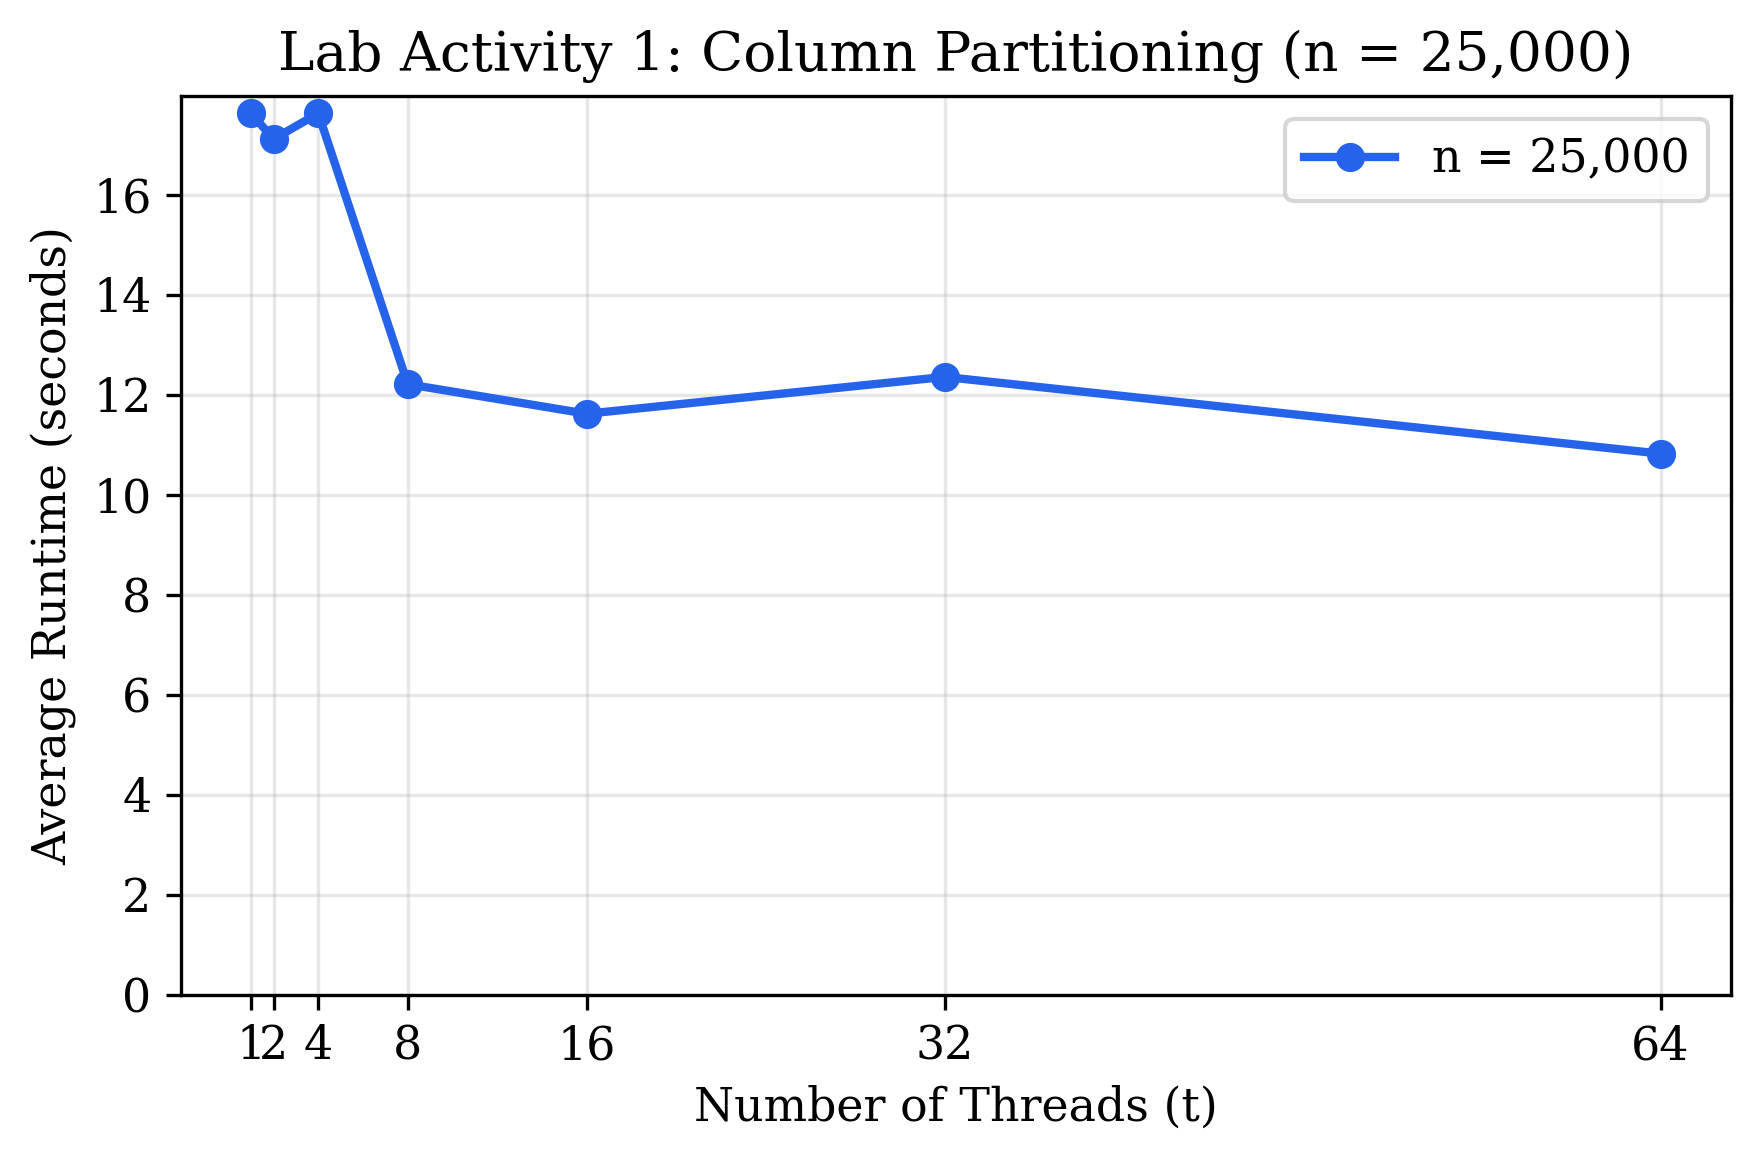
\includegraphics[width=\linewidth]{data/act1_graph.png}
    \caption{Lab Activity 1: Thread count vs. average runtime ($n=25{,}000$, column partitioning).}
    \label{fig:act1_graph}
\end{figure}

\begin{figure}[H]
    \centering
    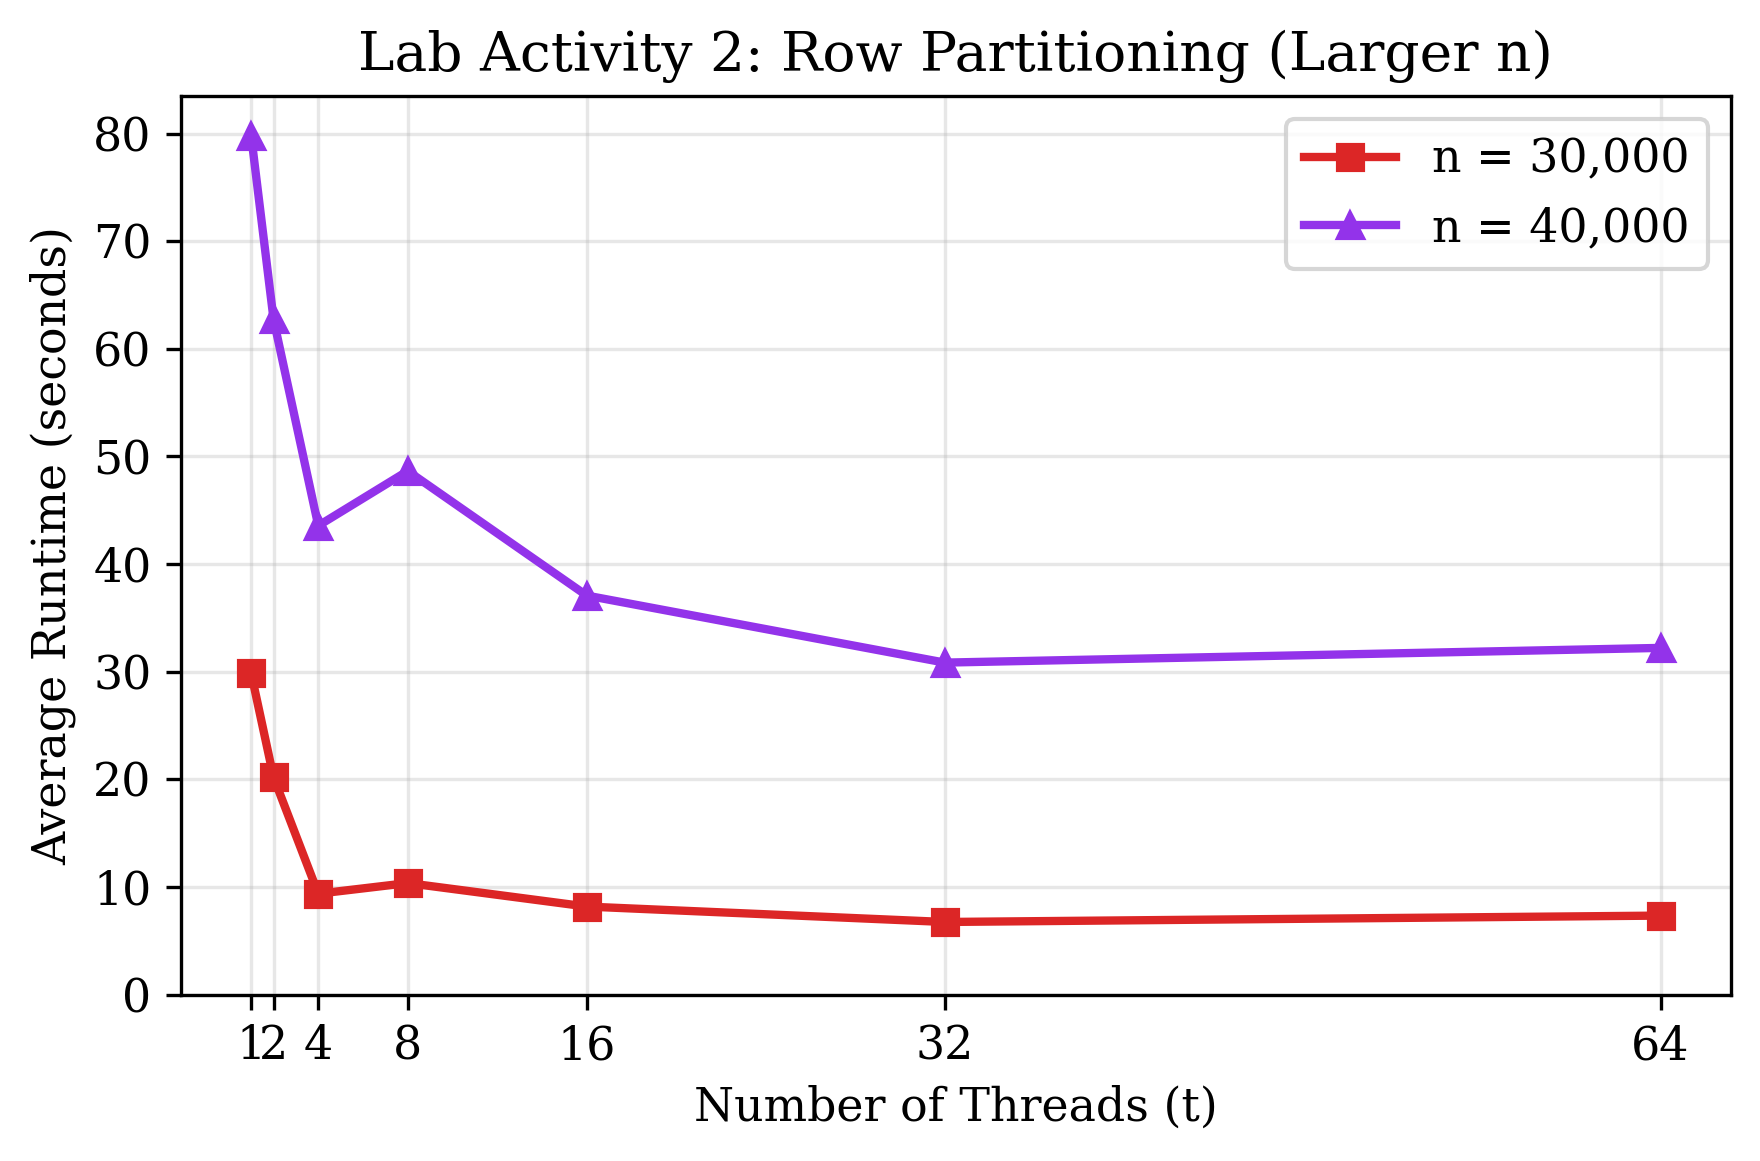
\includegraphics[width=\linewidth]{data/act2_graph.png}
    \caption{Lab Activity 2: Thread count vs. average runtime ($n=30{,}000$ and $n=40{,}000$, row partitioning).}
    \label{fig:act2_graph}
\end{figure}

\begin{figure}[H]
    \centering
    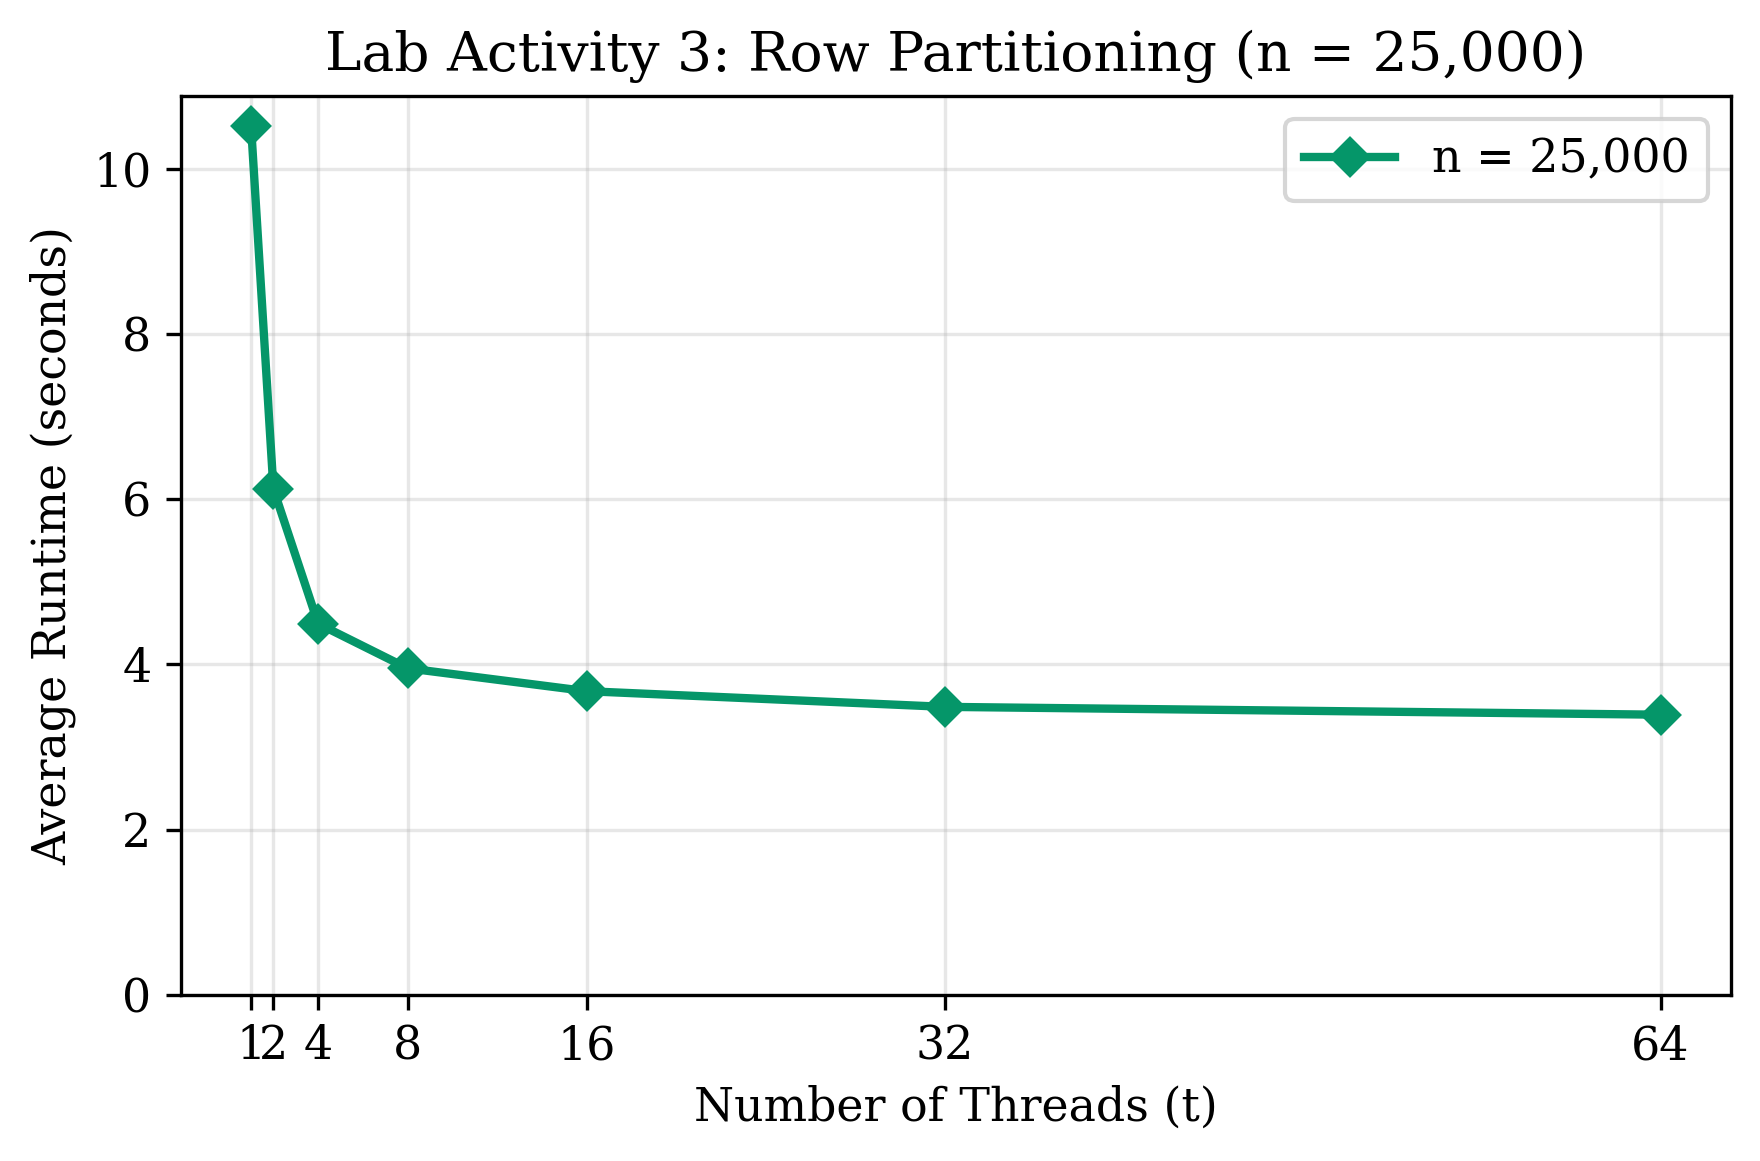
\includegraphics[width=\linewidth]{data/act3_graph.png}
    \caption{Lab Activity 3: Thread count vs. average runtime ($n=25{,}000$, row partitioning).}
    \label{fig:act3_graph}
\end{figure}

% SECTION 3
\section{Results and Discussion}

This section presents the findings of the experimental evaluation and addresses each research question systematically.

\subsection{RQ1: Parallel Complexity with $n$ Concurrent Processes}

\textbf{Research Question 1:} What do you think is the complexity of solving the MMT of the columns in an $n \times n$ square matrix $X$ when using $n$ concurrent processes?

With $n$ concurrent processes and the obvious assignment of one column per process, each process independently normalizes a single column. Normalizing one column requires scanning all $m = n$ rows to find the minimum and maximum ($O(n)$ operations), then scanning all $n$ rows again to apply the transformation ($O(n)$ operations). Therefore, each process performs $O(n)$ work.

Since all $n$ processes execute concurrently, the \textbf{parallel time complexity} is:

\begin{equation}
T_{\text{parallel}} = O(n)
\end{equation}

It is important to note that the \textbf{total work} across all processes remains $O(n^2)$, as each of the $n$ processes performs $O(n)$ operations. Parallelism does not reduce the total amount of computation; it distributes the work so that the wall-clock time is reduced.

\subsection{RQ2: Complexity with Fewer Concurrent Processes}

\textbf{Research Question 2:} What about $n/2$, $n/4$, $n/8$, and $n/m$ concurrent processes?

As the number of concurrent processes decreases, each process handles more columns. The table below summarizes the analysis:

\begin{table}[H]
    \centering
    \caption{Complexity Analysis for Varying Process Counts}
    \label{tab:complexity}
    \footnotesize
    \begin{tabular}{|c|c|c|c|}
        \hline
        \textbf{Processes} & \textbf{Cols/Process} & \textbf{Work/Process} & \textbf{Parallel Time} \\
        \hline
        $n$   & 1 & $O(n)$   & $O(n)$   \\
        \hline
        $n/2$ & 2 & $O(2n)$  & $O(n)$   \\
        \hline
        $n/4$ & 4 & $O(4n)$  & $O(n)$   \\
        \hline
        $n/8$ & 8 & $O(8n)$  & $O(n)$   \\
        \hline
        $n/m$ ($=1$) & $n$ & $O(n^2)$ & $O(n^2)$ \\
        \hline
    \end{tabular}
\end{table}

For $n/2$, $n/4$, and $n/8$ processes, each process handles a constant number of columns (2, 4, and 8, respectively). Since these constants are absorbed by asymptotic notation, the work per process remains $O(n)$ and the parallel time remains $O(n)$.

At $n/m$ concurrent processes, where $m = n$ for a square matrix, we have $n/m = 1$ process --- the serial case. A single process handles all $n$ columns, yielding $O(n^2)$ time.

The process assignment remains obvious in all cases: simply divide the $n$ columns into contiguous blocks of $n / p$ columns each, where $p$ is the number of processes. Since each column's normalization is independent of every other column, no inter-process communication is required regardless of the number of processes.

\subsection{RQ3: Threaded $t = 1$ vs. Serial LRP01}

\textbf{Research Question 3:} Why do you think that $t = 1$ will be a little bit higher than the average that was obtained in LRP01?

The LRP01 serial implementation for $n = 20{,}000$ averaged approximately 19.57 seconds. While a direct comparison at the same $n$ is not available in our data, the threaded implementation at $t = 1$ inherently carries overhead that the pure serial version does not:

\begin{enumerate}
    \item \textbf{Thread creation and joining}: Even with $t = 1$, the program invokes \texttt{pthread\_create()} and \texttt{pthread\_join()}, which involve system calls to manage a kernel-level thread. The serial LRP01 implementation simply calls \texttt{mmt()} directly --- a function call with no kernel involvement.
    
    \item \textbf{Transpose overhead}: The threaded implementation performs two transpose passes ($O(n^2)$ each) to convert from column-major to row-major access. These two passes are included in the timed section. The serial LRP01 did not perform any such transposition.
    
    \item \textbf{Timing mechanism}: The threaded implementation uses \texttt{clock\_gettime(CLOCK\_MONOTONIC)} (wall-clock time), whereas LRP01 used \texttt{clock()} (CPU time). Wall-clock time includes time the process spends waiting for the OS scheduler, context switches, and other system activity, which can be slightly higher.
\end{enumerate}

These combined overheads account for the small increase in runtime when $t = 1$ compared to the pure serial LRP01 baseline.

\subsection{RQ4: Row Partitioning ($n/t \times n$)}

\textbf{Research Question 4:} What will happen if we divide $X$ into $n/t \times n$ submatrices instead?

Dividing the matrix into $n/t \times n$ submatrices means each thread receives $n/t$ contiguous \textbf{rows} but all $n$ columns. This creates a fundamental problem: to normalize column $j$, a thread needs the minimum and maximum across \textit{all} $n$ rows of that column. However, each thread only has access to $n/t$ rows. No single thread possesses sufficient information to independently perform the normalization.

To arrive at the same answer, a \textbf{two-phase approach} is required:

\begin{enumerate}
    \item \textbf{Phase 1 --- Local Min/Max}: Each of the $t$ threads scans its $n/t$ rows and computes a local minimum and local maximum for every column $j$. This produces $t$ arrays of local minima and $t$ arrays of local maxima.
    
    \item \textbf{Reduce}: The main thread (serially) merges the $t$ local min arrays into a single global minimum per column, and similarly for the maximum. This reduction step iterates over $t \times n$ values.
    
    \item \textbf{Phase 2 --- Normalize}: The threads are respawned (or signaled via a barrier). Each thread normalizes its $n/t$ rows using the global min/max values, which are now shared read-only data.
\end{enumerate}

The tradeoff compared to column partitioning is:
\begin{itemize}
    \item \textbf{Advantage}: Row-wise access is inherently cache-friendly in C's row-major layout, so no transpose is needed.
    \item \textbf{Disadvantage}: The algorithm requires synchronization between the two phases (a barrier or two rounds of thread creation/join), and the serial reduce step adds $O(t \times n)$ overhead.
\end{itemize}

This row-partitioned approach was implemented as \texttt{lab02\_row.c} and evaluated in Lab Activity 3.

\subsection{Lab Activity 1: Column Partitioning Results}

Table~\ref{tab:act1_results} presents the results for $n = 25{,}000$ with the column-partitioned threaded program. The average runtime decreases from 17.63 seconds at $t = 1$ to 10.82 seconds at $t = 64$, representing a speedup of approximately $1.63\times$.

The improvement is moderate rather than dramatic. Ideally, doubling the thread count should halve the runtime, but several factors limit scaling:

\begin{itemize}
    \item The two transpose passes ($O(n^2)$ each) are serial overhead that does not benefit from additional threads.
    \item Memory bandwidth saturation: as more threads compete for the shared memory bus, each thread's effective memory throughput decreases.
    \item Thread management overhead: \texttt{pthread\_create/join} has fixed per-thread cost that becomes proportionally significant when per-thread work is small.
\end{itemize}

% TODO: Describe the graph observations once the graph is generated:
% The graph of $t$ versus Average Runtime shows a generally decreasing trend,
% with diminishing returns beyond $t = 16$. Going as far as $t = n$ (25,000 threads)
% would be counterproductive due to thread creation overhead dominating the minimal
% per-thread work. Practical limits appear around $t = n/4$ to $t = n/8$ for this
% matrix size.

\subsection{Lab Activity 2: Larger Matrix Sizes}

Lab Activity 2 uses the row-partitioned program (\texttt{lab02\_row}) to evaluate performance at larger matrix sizes, following from the row partitioning approach described in RQ4.

Table~\ref{tab:act2_30k} shows the results for $n = 30{,}000$. The row-partitioned program maintains good scaling behavior: the average runtime decreases from 29.85 seconds at $t = 1$ to 6.75 seconds at $t = 32$, a speedup of $4.42\times$. This is significantly better scaling than the column-partitioned program achieved at $n = 25{,}000$ ($1.63\times$), confirming the advantage of cache-friendly row-wise access.

Table~\ref{tab:act2_40k} shows the results for $n = 40{,}000$. Despite requiring approximately 12.8 GB of RAM (exceeding the 8 GB of physical memory), the program was able to execute by utilizing swap space. The runtimes are significantly higher and more variable due to heavy swap usage, but threading still provides a meaningful speedup: from 79.80 seconds at $t = 1$ to 30.85 seconds at $t = 32$ ($2.59\times$). The reduced scaling efficiency compared to $n = 30{,}000$ is attributable to swap-induced I/O latency, which creates a memory bandwidth bottleneck that limits the benefit of additional threads.

As shown in Table~\ref{tab:act2_failed}, the program was unable to execute for $n \geq 50{,}000$. An $n \times n$ matrix of \texttt{double} values (8 bytes each) requires $8n^2$ bytes of memory:
\begin{itemize}
    \item $n = 50{,}000$: $50{,}000^2 \times 8 \approx 20.0$ GB
    \item $n = 100{,}000$: $100{,}000^2 \times 8 \approx 80.0$ GB
\end{itemize}

These exceed the system's combined physical and virtual memory capacity, causing the operating system to terminate the process. Threading does not alleviate this constraint, as all threads share the same address space and the same matrix resides entirely in memory regardless of thread count.

To process larger matrices, one would need to increase physical RAM, use single-precision \texttt{float} (halving memory), or employ out-of-core algorithms that process the matrix in blocks stored on disk.

\subsection{Lab Activity 3: Row Partitioning Results}

Table~\ref{tab:act3_results} presents the results for $n = 25{,}000$ with the
row-partitioned threaded program. The average runtime decreases from 10.525 seconds
at $t = 1$ to 3.391 seconds at $t = 64$, representing a speedup of approximately
$3.10\times$ --- nearly twice the speedup achieved by column partitioning
($1.63\times$) at the same matrix size and thread count.

Several factors explain why row partitioning outperforms column partitioning here:

\begin{itemize}
    \item \textbf{Cache-friendly access}: In C's row-major memory layout, row
    partitioning accesses elements sequentially within each row, maximizing
    spatial locality. Column partitioning, even with the transpose trick, still
    incurs two $O(n^2)$ transpose passes that thrash the cache.

    \item \textbf{No transpose overhead}: The column-partitioned implementation
    includes two full matrix transposes within the timed region. Row partitioning
    eliminates this entirely, reducing the serial component of the workload.

    \item \textbf{Better scaling}: Row partitioning scales more consistently
    from $t = 1$ through $t = 8$, with roughly halving of runtime from
    $t = 1$ (10.525s) to $t = 2$ (6.126s) to $t = 4$ (4.493s) to $t = 8$
    (3.953s). Beyond $t = 8$, diminishing returns set in as the serial reduce
    step and thread management overhead dominate the shrinking per-thread workload.
\end{itemize}

The tradeoff is the added algorithmic complexity: row partitioning requires two
rounds of thread creation/joining and a serial $O(t \times n)$ reduction step,
whereas column partitioning uses a single round of threads. However, the
elimination of transpose overhead and the superior cache behavior more than
compensate, yielding a significantly faster result in practice.

% SECTION 4
\section{Conclusion}

This study extended the serial MMT implementation from LRP01 into a threaded program and investigated two partitioning strategies for distributing work across multiple threads. The investigation addressed all four research questions:

\begin{itemize}
    \item \textbf{RQ1}: With $n$ concurrent processes (one column each), the parallel time complexity is $O(n)$, as each process independently normalizes its column in $O(n)$ time.
    
    \item \textbf{RQ2}: With $n/2$, $n/4$, or $n/8$ processes, the parallel time remains $O(n)$ since each process handles a constant number of columns. At $n/m = 1$ (serial), the complexity returns to $O(n^2)$. The process assignment remains straightforward in all cases: contiguous blocks of columns.
    
    \item \textbf{RQ3}: The threaded implementation at $t = 1$ is slightly slower than the serial LRP01 due to thread creation/join overhead, two transpose passes, and differences in timing mechanisms (\texttt{clock\_gettime} vs. \texttt{clock}).
    
    \item \textbf{RQ4}: Row partitioning ($n/t \times n$) requires a two-phase approach --- local min/max computation, a serial reduce step, and then normalization --- because no single thread has access to a complete column. This introduces synchronization overhead but provides naturally cache-friendly row-wise memory access.
\end{itemize}

The experimental results for column partitioning at $n = 25{,}000$ showed a moderate speedup of $1.63\times$ at $t = 64$ relative to $t = 1$. Row partitioning achieved a significantly better speedup of $3.10\times$ at the same configuration, owing to cache-friendly access and the elimination of transpose overhead. Scaling to $n = 30{,}000$ and $n = 40{,}000$ using row partitioning was possible (with swap-induced latency at $n = 40{,}000$), while $n \geq 50{,}000$ exceeded available memory. These findings confirm that while threading can meaningfully reduce runtime for the MMT, the primary bottleneck at scale remains memory capacity rather than computational throughput, and the choice of partitioning strategy significantly impacts cache efficiency and parallel scaling.

% SECTION 5
\section{Responsible Use of AI}

\subsection{AI Usage Disclosure}
In the preparation of this report, AI tools (GitHub Copilot) were utilized to assist with paper outlining and organization, document formatting, technical analysis of cache behavior and threading overhead, and code optimization consultation.

\subsection{Justification for Responsible Use}
The core algorithm implementation in C, the design of the threading strategy, the execution of all experimental trials, the collection of runtime data, and the primary analysis of the results are the original work of the author. AI tools functioned solely as a technical thought partner and editorial assistant to enhance the presentation quality and provide theoretical context for observed phenomena. All AI-generated suggestions were critically reviewed, verified for accuracy, and adapted by the author before inclusion in this manuscript.

% APPENDICES
\appendices

\section{Source Code: Column Partitioning (\texttt{lab02.c})}

\begin{lstlisting}[style=ccode, caption={Threaded MMT with Column Partitioning}, label={lst:lab02}]
#include <stdio.h>
#include <stdlib.h>
#include <time.h>
#include <pthread.h>

// thread argument struct
typedef struct {
    double **matrix;
    int m;
    int col_start;
    int col_end;
} ThreadArg;

// create matrix function given n
double** createMat(int n){

    // allocate memory
    double **matrix = (double**)malloc(n*sizeof(double*));

    for (int i = 0; i < n; i++){
        matrix[i] = (double*)malloc(n*sizeof(double));
    }

    // fill in array
    
    for (int i = 0; i < n; i++){
        for (int j = 0; j < n; j++){
            matrix[i][j] =  (double)(rand() % 100 + 1);
        }
    }

    return matrix;
}

// transpose matrix in-place
void transpose(double **matrix, int n){
    for (int i = 0; i < n; i++){
        for (int j = i + 1; j < n; j++){
            double tmp = matrix[i][j];
            matrix[i][j] = matrix[j][i];
            matrix[j][i] = tmp;
        }
    }
}

// mmt function - normalizes columns 
// [col_start, col_end) of the matrix
// After transpose, columns become rows, 
// so we iterate rows for cache efficiency
void mmt(double **matrix, int m, 
    int col_start, int col_end){

    for (int j = col_start; j < col_end; j++){

        // after transpose, column j is now row j
        double col_min = matrix[j][0];
        double col_max = matrix[j][0];

        for (int i = 1; i < m; i++){
            if (matrix[j][i] > col_max){
                col_max = matrix[j][i];
            }
            if (matrix[j][i] < col_min){
                col_min = matrix[j][i];
            }
        }

        // normalize (row j in transposed 
        // = column j in original)
        for (int i = 0; i < m; i++){
            if (col_max - col_min != 0){
                matrix[j][i] = 
                    (matrix[j][i] - col_min)
                    /(col_max - col_min);
            }
        }
    }
}

// threaded mmt wrapper
void* mmtThread(void *arg){

    ThreadArg *targ = (ThreadArg*)arg;

    // call mmt on this thread's column slice
    mmt(targ->matrix, targ->m, 
        targ->col_start, targ->col_end);

    return NULL;
}

// main function
int main(){
    srand(time(NULL));

    int n, t;
    scanf("%d", &n);
    scanf("%d", &t);

    // create random n x n matrix
    double **matrix = createMat(n);

    // allocate thread arrays
    pthread_t *threads = 
        (pthread_t*)malloc(t * sizeof(pthread_t));
    ThreadArg *args = 
        (ThreadArg*)malloc(t * sizeof(ThreadArg));

    // divide X into t submatrices of size 
    // n x n/t each (x1, x2, ..., xt)
    int cols_per_thread = n / t;
    int remainder = n % t;

    // time before
    struct timespec time_before, time_after;
    clock_gettime(CLOCK_MONOTONIC, &time_before);

    // transpose so columns become rows
    transpose(matrix, n);

    // create t threads
    int col_offset = 0;
    for (int i = 0; i < t; i++){
        int cols = cols_per_thread 
            + (i < remainder ? 1 : 0);
        args[i].matrix = matrix;
        args[i].m = n;
        args[i].col_start = col_offset;
        args[i].col_end = col_offset + cols;
        col_offset += cols;

        pthread_create(&threads[i], NULL, 
            mmtThread, &args[i]);
    }

    // join all threads
    for (int i = 0; i < t; i++){
        pthread_join(threads[i], NULL);
    }

    // transpose back to original layout
    transpose(matrix, n);

    // time after
    clock_gettime(CLOCK_MONOTONIC, &time_after);

    double time_elapsed = 
        (time_after.tv_sec - time_before.tv_sec)
        + (time_after.tv_nsec - time_before.tv_nsec) 
        / 1e9;

    printf("%.6f\n", time_elapsed);

    // free memory (contiguous block)
    free(matrix[0]);
    free(matrix);
    free(threads);
    free(args);

    return 0;
}
\end{lstlisting}

\section{Source Code: Row Partitioning (\texttt{lab02\_row.c})}

\begin{lstlisting}[style=ccode, caption={Threaded MMT with Row Partitioning}, label={lst:lab02_row}]
#include <stdio.h>
#include <stdlib.h>
#include <time.h>
#include <pthread.h>

// thread argument struct for row partitioning
typedef struct {
    double **matrix;
    int n;
    int row_start;
    int row_end;
    double *local_min;
    double *local_max;
    double *global_min;
    double *global_max;
} ThreadArg;

// create matrix function given n
double** createMat(int n){

    // allocate memory
    double **matrix = (double**)malloc(n*sizeof(double*));

    for (int i = 0; i < n; i++){
        matrix[i] = (double*)malloc(n*sizeof(double));
    }

    // fill in array
    
    for (int i = 0; i < n; i++){
        for (int j = 0; j < n; j++){
            matrix[i][j] = (double)(rand() % 100 + 1);
        }
    }

    return matrix;
}

// phase 1: find local min and max for each column 
// within this thread's chunk of rows
void* mmtPhase1(void *arg){

    ThreadArg *targ = (ThreadArg*)arg;
    double **matrix = targ->matrix;
    int n = targ->n;
    int row_start = targ->row_start;
    int row_end = targ->row_end;
    double *local_min = targ->local_min;
    double *local_max = targ->local_max;

    // initialize from first row in chunk
    for (int j = 0; j < n; j++){
        local_min[j] = matrix[row_start][j];
        local_max[j] = matrix[row_start][j];
    }

    // scan remaining rows
    for (int i = row_start + 1; i < row_end; i++){
        for (int j = 0; j < n; j++){
            if (matrix[i][j] > local_max[j]){
                local_max[j] = matrix[i][j];
            }
            if (matrix[i][j] < local_min[j]){
                local_min[j] = matrix[i][j];
            }
        }
    }

    return NULL;
}

// phase 2: normalize using global min/max
void* mmtPhase2(void *arg){

    ThreadArg *targ = (ThreadArg*)arg;
    double **matrix = targ->matrix;
    int n = targ->n;
    int row_start = targ->row_start;
    int row_end = targ->row_end;
    double *global_min = targ->global_min;
    double *global_max = targ->global_max;

    for (int i = row_start; i < row_end; i++){
        for (int j = 0; j < n; j++){
            if (global_max[j] - global_min[j] != 0){
                matrix[i][j] = 
                    (matrix[i][j] - global_min[j])
                    /(global_max[j] - global_min[j]);
            }
        }
    }

    return NULL;
}

// main function
int main(){
    srand(time(NULL));

    int n, t;
    scanf("%d", &n);
    scanf("%d", &t);

    // create random n x n matrix
    double **matrix = createMat(n);

    // allocate thread arrays
    pthread_t *threads = 
        (pthread_t*)malloc(t * sizeof(pthread_t));
    ThreadArg *args = 
        (ThreadArg*)malloc(t * sizeof(ThreadArg));

    // allocate per-thread local min/max arrays
    double **all_local_min = 
        (double**)malloc(t * sizeof(double*));
    double **all_local_max = 
        (double**)malloc(t * sizeof(double*));
    for (int i = 0; i < t; i++){
        all_local_min[i] = 
            (double*)malloc(n * sizeof(double));
        all_local_max[i] = 
            (double*)malloc(n * sizeof(double));
    }

    // allocate global min/max arrays
    double *global_min = 
        (double*)malloc(n * sizeof(double));
    double *global_max = 
        (double*)malloc(n * sizeof(double));

    // partition rows across t threads
    int rows_per_thread = n / t;
    int remainder = n % t;

    // set up thread arguments
    int row_offset = 0;
    for (int i = 0; i < t; i++){
        int rows = rows_per_thread 
            + (i < remainder ? 1 : 0);
        args[i].matrix = matrix;
        args[i].n = n;
        args[i].row_start = row_offset;
        args[i].row_end = row_offset + rows;
        args[i].local_min = all_local_min[i];
        args[i].local_max = all_local_max[i];
        args[i].global_min = global_min;
        args[i].global_max = global_max;
        row_offset += rows;
    }

    // time before
    struct timespec time_before, time_after;
    clock_gettime(CLOCK_MONOTONIC, &time_before);

    // PHASE 1: find local min/max per thread
    for (int i = 0; i < t; i++){
        pthread_create(&threads[i], NULL, 
            mmtPhase1, &args[i]);
    }
    for (int i = 0; i < t; i++){
        pthread_join(threads[i], NULL);
    }

    // REDUCE: merge local into global min/max
    for (int j = 0; j < n; j++){
        global_min[j] = all_local_min[0][j];
        global_max[j] = all_local_max[0][j];
    }
    for (int i = 1; i < t; i++){
        for (int j = 0; j < n; j++){
            if (all_local_min[i][j] < global_min[j])
                global_min[j] = all_local_min[i][j];
            if (all_local_max[i][j] > global_max[j])
                global_max[j] = all_local_max[i][j];
        }
    }

    // PHASE 2: normalize using global min/max
    for (int i = 0; i < t; i++){
        pthread_create(&threads[i], NULL, 
            mmtPhase2, &args[i]);
    }
    for (int i = 0; i < t; i++){
        pthread_join(threads[i], NULL);
    }

    // time after
    clock_gettime(CLOCK_MONOTONIC, &time_after);

    double time_elapsed = 
        (time_after.tv_sec - time_before.tv_sec)
        + (time_after.tv_nsec - time_before.tv_nsec) 
        / 1e9;

    printf("%.6f\n", time_elapsed);

    // free memory
    for (int i = 0; i < t; i++){
        free(all_local_min[i]);
        free(all_local_max[i]);
    }
    free(all_local_min);
    free(all_local_max);
    free(global_min);
    free(global_max);
    for (int i = 0; i < n; i++){
        free(matrix[i]);
    }
    free(matrix);
    free(threads);
    free(args);

    return 0;
}
\end{lstlisting}

% BIBLIOGRAPHY
\begin{thebibliography}{9}

\bibitem{drepper2007}
Drepper, U. (2007). \emph{What Every Programmer Should Know About Memory}. Red Hat, Inc. Retrieved from https://people.freebsd.org/\~{}lstewart/articles/cpumemory.pdf

\bibitem{cornell2023}
Cornell Virtual Workshop. (2023). \emph{Cache-Friendly Code}. Cornell University Center for Advanced Computing. Retrieved from https://cvw.cac.cornell.edu/vector/coding\_cache

\bibitem{wikipedia_falsesharing}
Wikipedia. (2024). \emph{False sharing}. Retrieved from https://en.wikipedia.org/wiki/False\_sharing

\bibitem{geeksforgeeks2023}
GeeksforGeeks. (2023). \emph{Row-major order and column-major order in 2D arrays}. Retrieved from https://www.geeksforgeeks.org/row-major-order-and-column-major-order/

\bibitem{pthreads}
IEEE Std 1003.1. \emph{POSIX Threads}. The Open Group. Retrieved from https://pubs.opengroup.org/onlinepubs/9699919799/functions/pthread\_create.html

\end{thebibliography}

\end{document}
